\documentclass[aspectratio=169]{beamer}
\usepackage{will_handley}

\newcommand{\av}[2][1]{\left\langle #2\right\rangle_{#1}}

% Commands
% --------
% - \arxiv{arxiv number}
% - \cols{width}{lh column}{rh column}
% -  \begin{fig(left|right)}[fractional width (e.g 0.6) ]{name of image}
%        content of other column
%    \end{fig(left|right)}

% Talk details
% ------------
\title{Statistical methods in cosmology}
\subtitle{<+subtitle+>}
\date{12\textsuperscript{th} April 2022}

\begin{document}

\begin{frame}
    \titlepage
\end{frame}

\begin{frame}
    \frametitle{Lessons from the CMB}
    \begin{columns}
        \column{0.5\textwidth}
        \begin{itemize}
            \item 21cm global signal detection is superficially similar to detecting the primordial CMB.
            \item Both are attempted to detect tiny $\sim 10^{-5}$ cosmological signals hidden beneath a large ``uninteresting'' foreground.
            \item Both measurements are frustrated by complicated contaminants.
            \item Both are amenable to a Bayesian analysis.
        \end{itemize}
        \column{0.5\textwidth}
        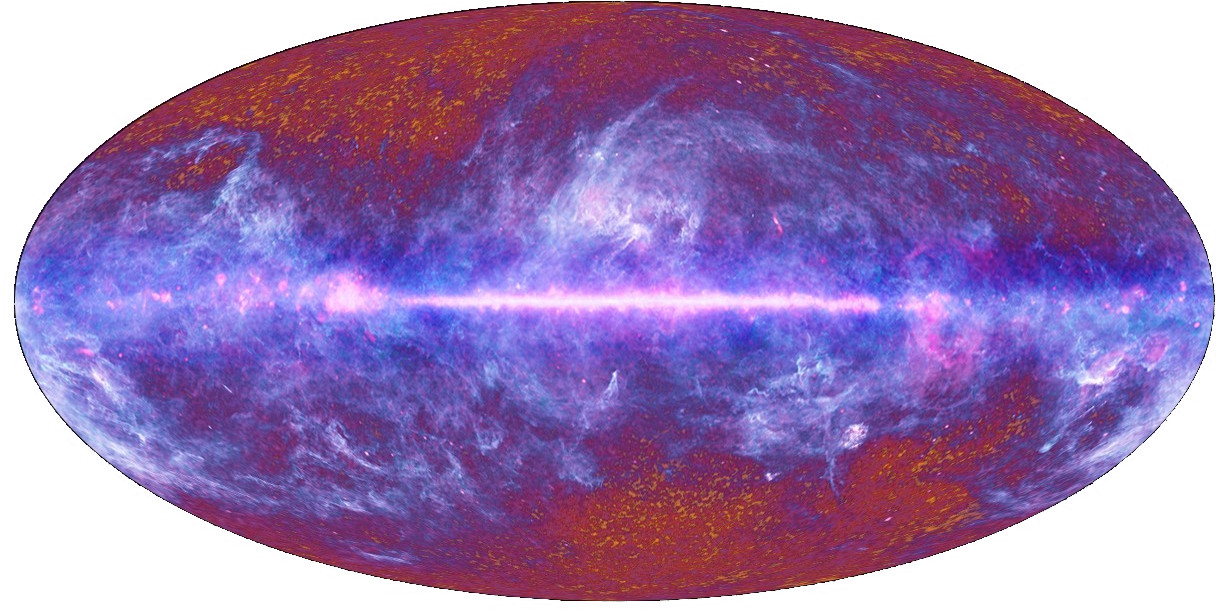
\includegraphics[width=\textwidth]{figures/9HXKAsNw5LtSRHFPWfeqiB.jpg}
        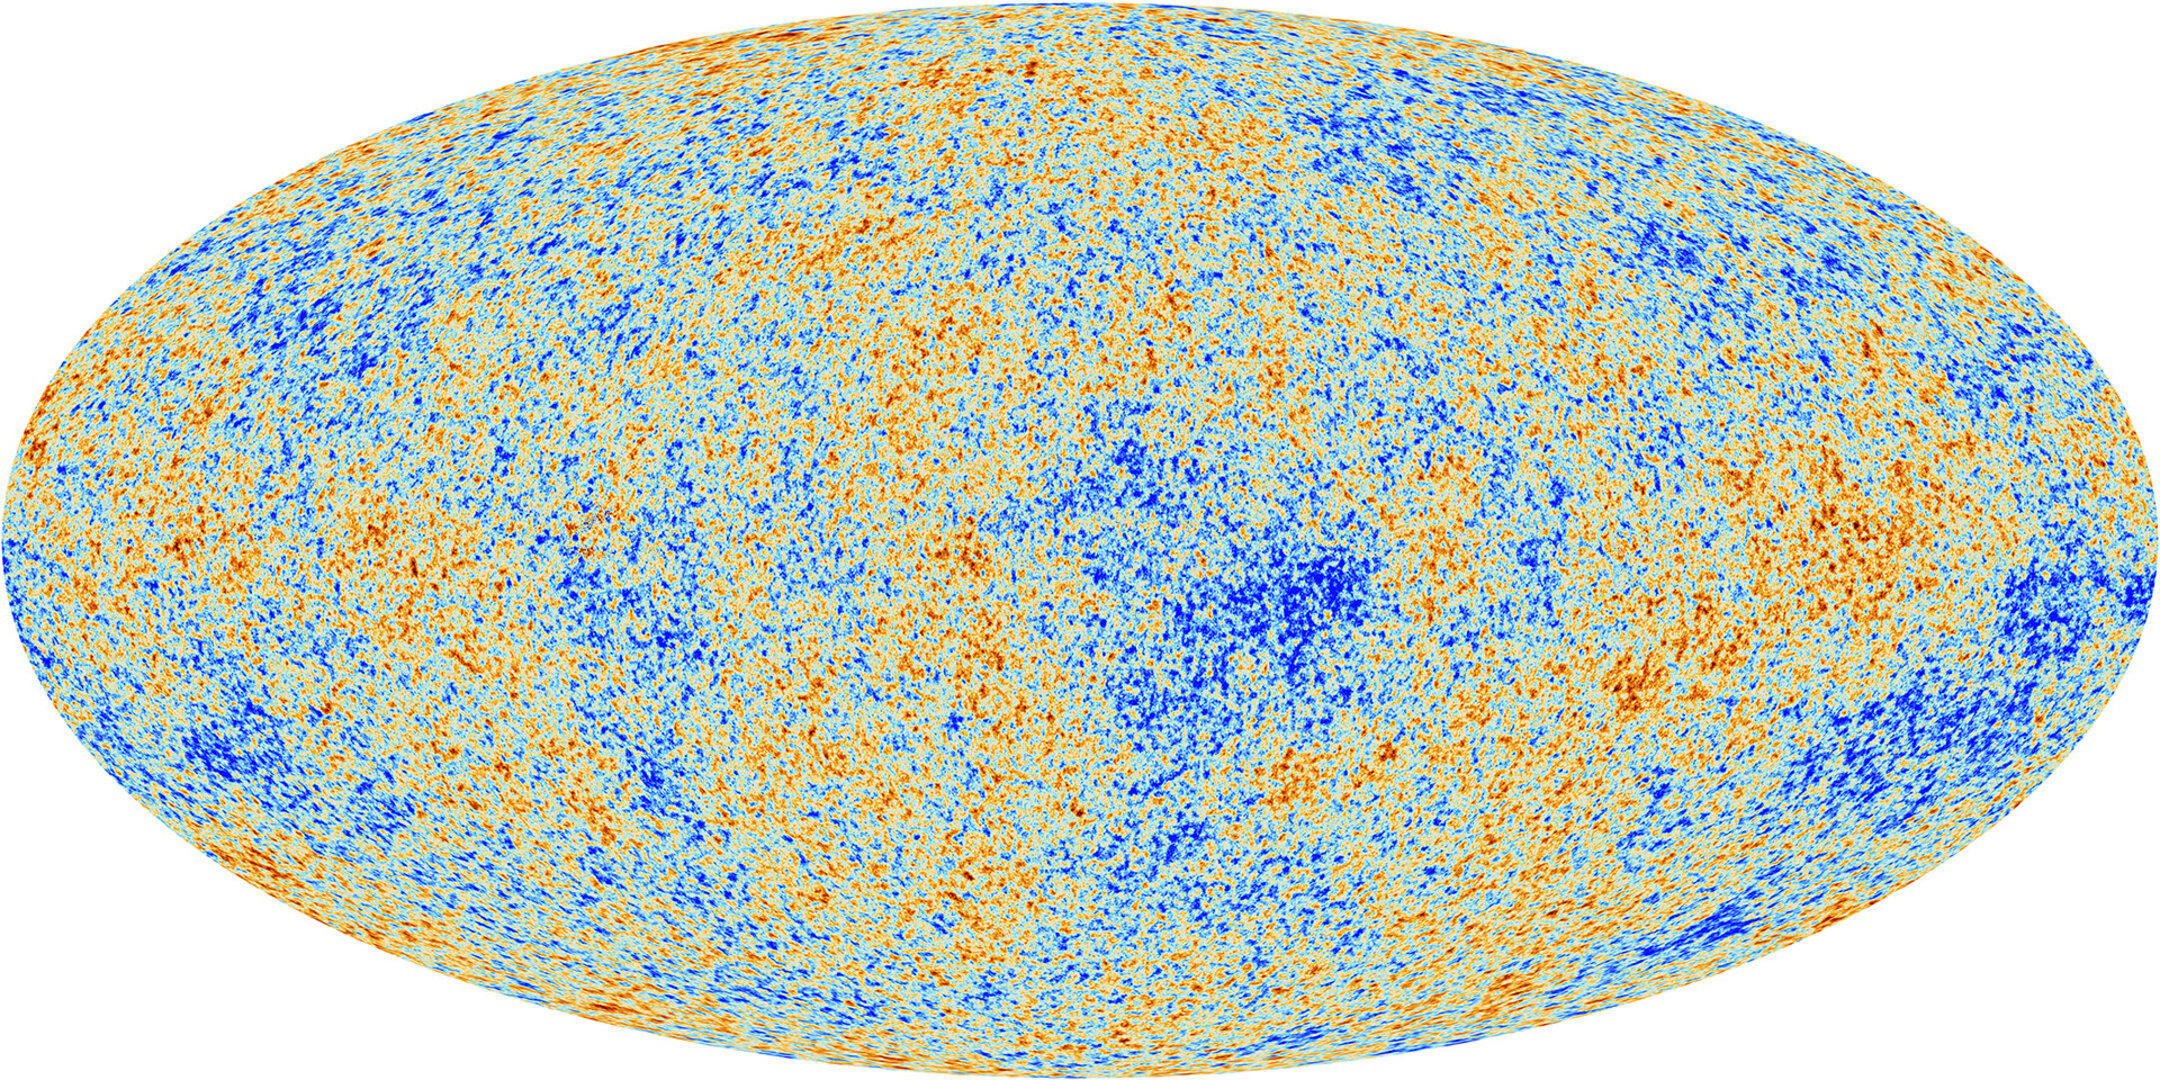
\includegraphics[width=\textwidth]{figures/Planck_satellite_cmb.jpg}

    \end{columns}
\end{frame}

\begin{frame}
    \frametitle{The three pillars of Bayesian inference}
    \begin{itemize}
        \item Parameter estimation: ``What do the data tell me about my model?'':
            \[ \C[0]{P(\theta|D,M)} = \frac{\C[2]{P(D|\theta,M)} \C[1]{P(\theta|M)}}{\C[3]{P(D|M)}}, \qquad \C[0]{\mathcal{P}} = \frac{\C[2]{\mathcal{L}} \times\C[1]{\pi}}{\C[3]{\mathcal{Z}}}, \qquad \C[0]{\text{Posterior}} = \frac{\C[2]{\text{Likelihood}} \times\C[1]{\text{Prior}}}{\C[3]{\text{Evidence}}}. \]
        \item Model comparison: ``Which model best fits the data?'':
            \[ \C[4]{P(M|D)} = \frac{\C[3]{P(D|M)} \C[5]{P(M)}}{\C[6]{P(D)}}, \qquad \frac{\C[3]{\mathcal{Z}_\mathcal{M}} \C[5]{\Pi_\mathcal{M}}}{\C[6]{\sum_m Z_m \Pi_m}}, \qquad \C[4]{\text{Model Posterior}} = \frac{\C[3]{\text{Evidence}} \times\C[5]{\text{Model Prior}}}{\C[6]{\text{Normalisation}}}.\]
        \item Tension quantification: ``Are datasets consistent within a given model?'' \arxiv{1902.04029}
        \[ \mathcal{R} = \frac{\mathcal{Z}_{AB}}{\mathcal{Z}_A\mathcal{Z}_\mathcal{B}}, \qquad \log\mathcal{S} = \av[\mathcal{P}_{AB}]{\log\mathcal{L}_{AB}}-\av[\mathcal{P}_{A}]{\log\mathcal{L}_{B}}-\av[\mathcal{P}_{B}]{\log\mathcal{L}_{B}}  \]
    \end{itemize}
\end{frame}

\begin{frame}
    \frametitle{Foregrounds and parametric models}
    <+Content+>
\end{frame}

\begin{frame}
    \frametitle{What is a model?}
\end{frame}

\begin{frame}
    \frametitle{Occam's Razor~\arxiv{2102.11511}}
    \begin{itemize}
        \item Bayesian inference quantifies Occam's Razor:
            \begin{itemize}
                \item \textit{``Entities are not to be multiplied without necessity''} \hfill --- William of Occam
                \item \textit{``Everything should be kept as simple as possible, but not simpler''} \hfill --- ``Albert Einstein''
            \end{itemize}
        %\item Consider the Evidence $\C[3]{\mathcal{Z}\equiv P(D|M)}$: 
        %    \begin{description}[Parameter estimation]
        %        \item [Parameter estimation] normalisation constant
        %        \item [Model comparison] critical update factor for \C[5]{model prior} to \C[4]{model posterior}
        %    \end{description}
        \item Properties of the evidence: rearrange Bayes' theorem for parameter estimation
            \[\C[0]{\mathcal{P}(\theta)} = \frac{\C[2]{\mathcal{L}(\theta)} \C[1]{\pi(\theta)}}{\C[3]{\mathcal{Z}}} \qquad\Rightarrow\qquad \C[3]{\log \mathcal{Z}} = \C[2]{\log\mathcal{L}(\theta)} - \log \frac{\C[0]{\mathcal{P}(\theta)}}{\C[1]{\pi(\theta)}} \]  
        \item Evidence is composed of a ``goodness of fit'' term  and ``Occam Penalty''
    \end{itemize}
    \begin{columns}[t]
        \column{0.5\textwidth}
    \begin{itemize}
        \item RHS true for all $\theta$. Take maximum value $\theta_\mathrm{max}$:
            \[
                \log \mathcal{Z} = -\chi_\mathrm{min}^2 - \text{Mackay penalty}
            \]
    \end{itemize}
        \column{0.5\textwidth}
    \begin{itemize}
        \item Be more Bayesian and take posterior average to get the ``Occam's razor equation''
            \[
                \boxed{
                    \log \mathcal{Z} = \av[\mathcal{P}]{\log\mathcal{L}} - \mathcal{D}_\mathrm{KL}
            }
            \]
    \end{itemize}
    \end{columns}
    \vfill
    \begin{itemize}
        \item Natural regularisation which penalises models with too many parameters.
    \end{itemize}
\end{frame}

\begin{frame}
    \frametitle{Kullback Liebler divergence}
    \begin{columns}
        \column{0.5\textwidth}
        \begin{itemize}
            \item The KL divergence between \C[1]{prior $\pi$} and \C[0]{posterior $\mathcal{P}$} is is defined as:
                \[\mathcal{D}_\mathrm{KL} = \av[\mathcal{P}]{\log\frac{\mathcal{P}}{\pi}} = \int \mathcal{P}(\theta) \log \frac{\mathcal{P}(\theta)}{\pi(\theta)}d\theta.\]
            \item Whilst not a distance, $\mathcal{D}=0$ when $\mathcal{P}=\pi$.
            \item Occurs in the context of machine learning as an objective function for training functions.
            \item In Bayesian stats it can be understood as a log-ratio of ``volumes'':
                \[ \mathcal{D}_\mathrm{KL} \approx \log \frac{V_\pi}{V_\mathrm{P}}.\]
                (this is exact for top-hat distributions).
        \end{itemize}
        \column{0.5\textwidth}
        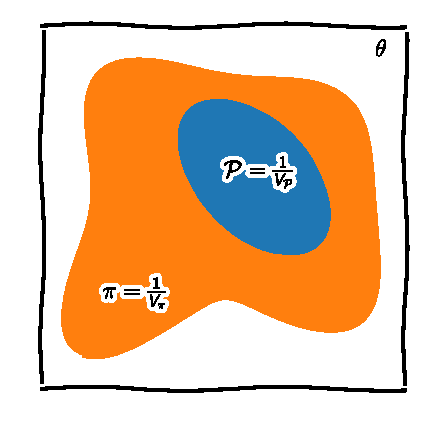
\includegraphics{figures/volumes.pdf}
    \end{columns}
\end{frame}

\begin{frame}
    \frametitle{Why do sampling?}
    <+Content+>
\end{frame}

\begin{frame}
    \frametitle{MCMC vs Nested Sampling}
    <+Content+>
\end{frame}

\begin{frame}
    \frametitle{Non-parametric reconstruction}
    <+Content+>
\end{frame}

\end{document}
